\def\year{2021}\relax
%File: formatting-instructions-latex-2021.tex
%release 2021.1
\documentclass[letterpaper]{article} % DO NOT CHANGE THIS
\usepackage{aaai21}  % DO NOT CHANGE THIS
\usepackage{times}  % DO NOT CHANGE THIS
\usepackage{helvet} % DO NOT CHANGE THIS
\usepackage{courier}  % DO NOT CHANGE THIS
\usepackage[hyphens]{url}  % DO NOT CHANGE THIS
\usepackage{graphicx} % DO NOT CHANGE THIS

% ADJUSTED BY AFM ----------------------------------------------------------
\usepackage{amsmath} % ENTERED BY AFM

\urlstyle{rm} % DO NOT CHANGE THIS
\def\UrlFont{\rm}  % DO NOT CHANGE THIS
\usepackage{natbib}  % DO NOT CHANGE THIS AND DO NOT ADD ANY OPTIONS TO IT
\usepackage{caption} % DO NOT CHANGE THIS AND DO NOT ADD ANY OPTIONS TO IT
\frenchspacing  % DO NOT CHANGE THIS
\setlength{\pdfpagewidth}{8.5in}  % DO NOT CHANGE THIS
\setlength{\pdfpageheight}{11in}  % DO NOT CHANGE THIS
\nocopyright
%PDF Info Is REQUIRED.
% For /Author, add all authors within the parentheses, separated by commas. No accents or commands.
% For /Title, add Title in Mixed Case. No accents or commands. Retain the parentheses.
\pdfinfo{
/Title (ML Assignment 1)
/Author (Anthony Menninger)
/TemplateVersion (2021.1)
} %Leave this
% /Title ()
% Put your actual complete title (no codes, scripts, shortcuts, or LaTeX commands) within the parentheses in mixed case
% Leave the space between \Title and the beginning parenthesis alone
% /Author ()
% Put your actual complete list of authors (no codes, scripts, shortcuts, or LaTeX commands) within the parentheses in mixed case.
% Each author should be only by a comma. If the name contains accents, remove them. If there are any LaTeX commands,
% remove them.

% DISALLOWED PACKAGES
% \usepackage{authblk} -- This package is specifically forbidden
% \usepackage{balance} -- This package is specifically forbidden
% \usepackage{color (if used in text)
% \usepackage{CJK} -- This package is specifically forbidden
% \usepackage{float} -- This package is specifically forbidden
% \usepackage{flushend} -- This package is specifically forbidden
% \usepackage{fontenc} -- This package is specifically forbidden
% \usepackage{fullpage} -- This package is specifically forbidden
% \usepackage{geometry} -- This package is specifically forbidden
% \usepackage{grffile} -- This package is specifically forbidden
% \usepackage{hyperref} -- This package is specifically forbidden
% \usepackage{navigator} -- This package is specifically forbidden
% (or any other package that embeds links such as navigator or hyperref)
% \indentfirst} -- This package is specifically forbidden
% \layout} -- This package is specifically forbidden
% \multicol} -- This package is specifically forbidden
% \nameref} -- This package is specifically forbidden
% \usepackage{savetrees} -- This package is specifically forbidden
% \usepackage{setspace} -- This package is specifically forbidden
% \usepackage{stfloats} -- This package is specifically forbidden
% \usepackage{tabu} -- This package is specifically forbidden
% \usepackage{titlesec} -- This package is specifically forbidden
% \usepackage{tocbibind} -- This package is specifically forbidden
% \usepackage{ulem} -- This package is specifically forbidden
% \usepackage{wrapfig} -- This package is specifically forbidden
% DISALLOWED COMMANDS
% \nocopyright -- Your paper will not be published if you use this command
% \addtolength -- This command may not be used
% \balance -- This command may not be used
% \baselinestretch -- Your paper will not be published if you use this command
% \clearpage -- No page breaks of any kind may be used for the final version of your paper
% \columnsep -- This command may not be used
% \newpage -- No page breaks of any kind may be used for the final version of your paper
% \pagebreak -- No page breaks of any kind may be used for the final version of your paperr
% \pagestyle -- This command may not be used
% \tiny -- This is not an acceptable font size.
% \vspace{- -- No negative value may be used in proximity of a caption, figure, table, section, subsection, subsubsection, or reference
% \vskip{- -- No negative value may be used to alter spacing above or below a caption, figure, table, section, subsection, subsubsection, or reference

\setcounter{secnumdepth}{0} %May be changed to 1 or 2 if section numbers are desired.

% The file aaai21.sty is the style file for AAAI Press
% proceedings, working notes, and technical reports.
%

% Title

% Your title must be in mixed case, not sentence case.
% That means all verbs (including short verbs like be, is, using,and go),
% nouns, adverbs, adjectives should be capitalized, including both words in hyphenated terms, while
% articles, conjunctions, and prepositions are lower case unless they
% directly follow a colon or long dash


%Example, Single Author, ->> remove \iffalse,\fi and place them surrounding AAAI title to use it
\title{
Machine Learning - CS 7641
Assignment 1
	
}
\author {
    % Author
    Anthony Menninger \\
}

\affiliations{
    Georgia Tech OMSCS Program \\
    tmenninger@gatech.edu

}

\begin{document}

\maketitle

\begin{abstract}
FILL IN?
\end{abstract}

\section{Introduction}


\section{Data Sets}

The first data set is from 1994 and 1995 current population surveys conducted by the U.S. Census Bureau [1] from the UC Irvine Machine learning site.  The classification task is to determine if the user type for each instance has an income above \$50,000 or below (\$94,000 in today's dollars).  The 1994 median annual salary was \$16,000 (2020 median salary was \$34,600) 

There are 40 usable features, with both continuous features, such as age, and discrete, such as married status or sex.  The training set has 199,523 instances and the test set has 99,762 instances.  Because many of the features in the file are string based, I created transformed instances using the sklearn preprocessing LabelEncoder to translate discrete string values into consistent numeric values.  This was necessary for algorithms that only used numeric features. I chose this data set because it seemed relatively large and I expect somewhat noisy with a smallish number of features.  

The second data set is The MNIST Database of Handwritten Digits [2].  This consists of instances of 28 X 28 greyscale images of the digits 0-9.  The only transformation needed was that each of these images was flattened, creating 784 features, one for each pixel.  There are 60,000 training instances and 10,000 test instances.  I chose this because it is a good comparison to the first data set, with a very different type of data (images), which leads to significantly more features (784).  In addition, each of the features can be thought of as related to each other, as they are all positional in a two dimensional grid, while the first data set features do not have any necessary relation between themselves ie:  age is not related to sex.  

ADD DISCUSION ON BALANCE OF LABELS - CENSUS CAN GET GOOD SCORE WITH JUST 0

\section{Decision Trees}
Decision Trees. For the decision tree, you should implement or steal a decision tree algorithm (and by "implement or steal" I mean "steal"). Be sure to use some form of pruning. You are not required to use information gain (for example, there is something called the GINI index that is sometimes used) to split attributes, but you should describe whatever it is that you do use.

I used the DecisionTreeClassifier algorithm from the sklearn library.  By default, this uses a GINI index to split the data.  It was possible to use an information gain entropy for splitting, but this did not make a meaningful difference in results for the datasets so the GINI index was used.  A key aspect of sklearn is that it only accepts numeric data for features and treats all features as continuous.  Because of this, a feature can appear in multiple nodes within the same path, with different thresholds.  It also means this is a binary tree, with each node having only two edges.  Other decision tree implementations might allow for discreet features, meaning a feature could only appear once in any tree path and the tree might not be binary.  

sklearn also uses a randomizing element, which means that given the same set of data, it may produce different results each run.  In order to produce consistent, repeatable results, the random state setting was set to a fixed value to produce the same results each time.

I also used the sklearn Cross Validation module for estimating the best solution without using the test data.  This was then confirmed by reviewing the test data.

\begin{figure}[htb]
\centering
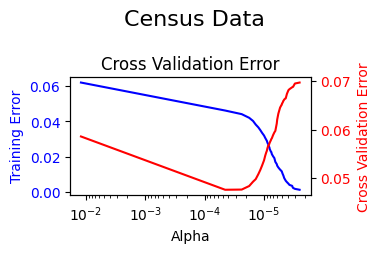
\includegraphics[width=2.75in]{figures/Census_Data_decision_tree_cross_validation.png}
\caption{Census Data Cross Validation.  The cross validation error starts to rise as the decision tree starts to over fit.  The best cross validation $\alpha$ value of 0.0000153 had a test accuracy of 95.24\%, which was very close to the actual best testing score of 95.30\%. }
\label{fig:census_data_decision_tree_cross_validation}
\end{figure}

\begin{figure}[htb]
\centering
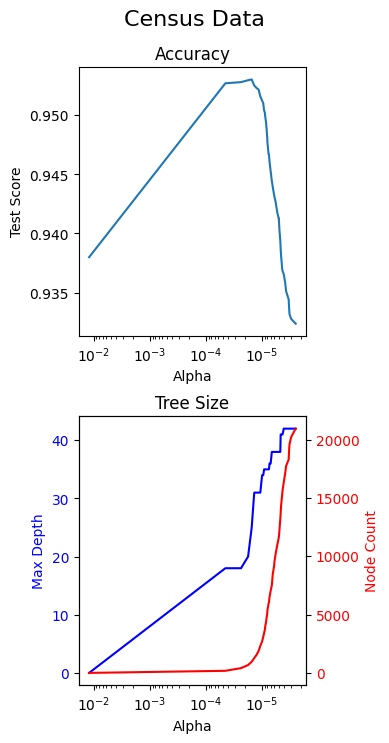
\includegraphics[width=2.75in, height=4in]{figures/Census_Data_decision_tree.png}
\caption{Census Data Decision Tree:  The right side of the upper chart shows overfitting as the pruning is reduced and the number of nodes and tree depth increases.  An unusual aspect is the left side of the chart shows very high accuracy with very few nodes.  This stems from one feature being highly correlated to the labeled output.}
\label{fig:census_data_decision_tree}
\end{figure}


To prune the tree, sklearn uses a minimal cost-complexity setting.  Each node in a tree has an $\alpha$ value which measures the node misclassifications minus leaves misclassifications divided by the number of leaf nodes.  The DecisionTreeClassifier then takes an $\alpha$ minimum setting, pruning all subtrees with a lower $\alpha$.   For both datasets, an accuracy curve was created by fitting the tree with different $\alpha$ values.  

For both data sets, I also performed cross validation to use the training set only to determine the best $\alpha$ parameter, with a 5 fold setting (80\% of training data used for training, 20\% used for validation).  I would then use the test data at different $\alpha$ values to confirm the finding.

For the Census Data, Figure \ref{fig:census_data_decision_tree_cross_validation} shows the use of cross validation to estimate the best solution, in this case setting for $\alpha$, without using the test data.   The best cross validation $\alpha$ value of 0.0000153 had a test accuracy of 95.24\%, which was very close to the actual best testing score of 95.30\%.  Cross Validation provides a powerful tool for evaluation a given training set without reference to test data when available.

The Census Data, shown in Figure \ref{fig:census_data_decision_tree},  mostly shows the expected curve.  Accuracy improves as nodes are added, to a point, then accuracy declines due to over fitting as more nodes are added.  Alpha, the pruning constant, leaves more nodes in the tree as it is decreased.  The Census Data also showed a unique characteristic.  One of its features (Capital Losses), showed a very high correlation with the labeled output, Income above \$50k.  Thus, a one node tree already showed 94\% accuracy.  Figure \ref{fig:census_data_decision_tree} shows this, with the the left side of the chart with few nodes already having a very high accuracy.  


\begin{figure}[htb]
\centering
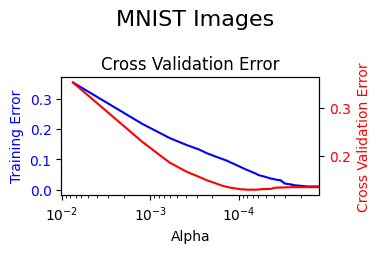
\includegraphics[width=2.75in]{figures/MNIST_Images_decision_tree_cross_validation.png}
\caption{MNIST Images Cross Validation Error:  The chart shows continual reduction in training error, while the Cross Validation error reaches a minimum at an $\alpha$ of 0.0000542 and then starts to rise.  This was very close to the best $\alpha$ found using the testing data. }
\label{fig:MNIST_Images_decision_tree_cross_validation}
\end{figure}

Figure \ref{fig:MNIST_Images_decision_tree_cross_validation}  shows the cross validation error curves for the MNIST image data.  The best cross validation $\alpha$ value of 0.0000762 had a test accuracy of 87.18\%,  while the actual best testing score of 88.54\%.  This was a larger gap than found in the Census data, but still relatively close.

\begin{figure}[htb]
\centering
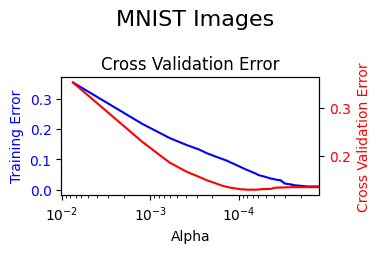
\includegraphics[width=2.75in]{figures/MNIST_Images_decision_tree_cross_validation.png}
\caption{MNIST Images Cross Validation Error:  The chart shows continual reduction in training error, while the Cross Validation error reaches a minimum at an $\alpha$ of 0.0000542 and then starts to rise.  This was very close to the best $\alpha$ found using the testing data. }
\label{fig:MNIST_Images_decision_tree_cross_validation}
\end{figure}

The MNIST image data, shown in Figure \ref{fig:MNIST_Images_decision_tree}, showed a more normal accuracy curve than the Census Data, with accuracy improving dramatically with added nodes until a maximum accuracy was reached, then accuracy declines due to over fitting.  The maximum accuracy achieved was 88.7\%, which was significantly below the census data.  A decision tree is looking at one pixel at a time, 
so small variations in position or size would be very challenging for this algorithm.  I think other classifiers, especially the neural network to better handle image data. 

\section{Neural Networks}
For the neural network, I used PyTorch with two hidden layers, the Adam optimizer and Linear layers.  I then adjusted the size of the layer, the learning rate, and epoch cycles to find the optimal settings.

In just the initial setup for the Census data, I quickly determined I would need to scale the data as the solver would often "blow up" with really large values.  I used the sklearn StandardScaler module, which removes the mean from each feature then applies a sigmoid function to create values from -1 to 1.  This is somewhat suspect for the categorical features, as there is not really a positional relationship, but it was still effective.  I also switched to using a 4 Fold Cross Validation model as I became more worried about the smaller data.

\begin{figure}[htb]
\centering
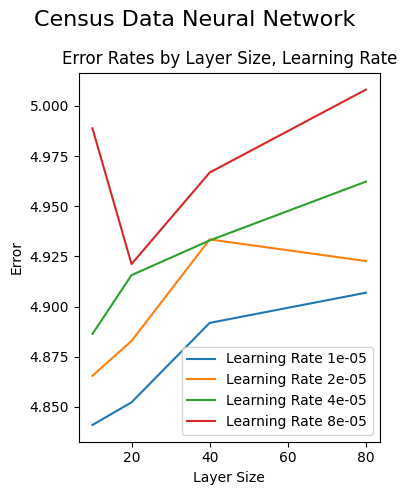
\includegraphics[width=2.75in, height=2.75in]{figures/Census_Data_Neural_Network_Error_Rates_by_Layer_Size__Learning_Rate_census.png}
\caption{Census Data Neural Network:  Review started to look for optimizing the neural network.  The lowest error is clearly shown for the smaller learning rate with the smaller network.   }
\label{fig:census_neural_network_start}
\end{figure}

 Figure \ref{fig:census_neural_network_start} clearly shows the preference for the smaller layer size and smaller learning rate, although the differences in absolute accuracy are quite small.  This is a victory still due to the very skewed dataset, with only ~6\% of the data being labeled positively.  The smaller layer size performance is straight out of the class lecture with regard to preferring simpler solutions.  I had expected larger layer sizes to be more effective.  The charts indicates that further exploration at the lower end was worthwhile.

\begin{figure}[htb]
\centering
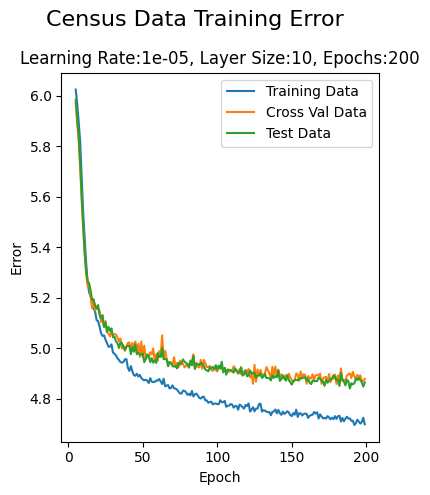
\includegraphics[width=2.75in, height=2.75in]{figures/Census_Data_Training_Error_Learning_Rate_chart_one.png}
\caption{Census Data Neural Network Training Error:  It shows that the cross validation error was very close to the real test data error and a good guide for decision making.  }
\label{fig:census_neural_network_error}
\end{figure}

Figure \ref{fig:census_neural_network_error} shows one of the best performing settings from the initial review.  It shows that the cross validation error was very close to the real test data error and a good guide for decision making.  The chart also doesn't clearly have a movement up of the cross validation error, indicating more epoch training may be beneficial

\section{References}
\begin{tabular}{l p{2.75in}}
\\
1 & Census Income (KDD). url: https://archive-beta.ics.uci.edu/ml/datasets/census+income+kdd.
\\
2 & The MNIST Database of Handwritten Digits. url: http://yann.lecun.com/exdb/mnist/.
\end{tabular}
\end{document}
